%%%% ijcai19.tex

\typeout{IJCAI-19 Instructions for Authors}

% These are the instructions for authors for IJCAI-19.

\documentclass{article}
\pdfpagewidth=8.5in
\pdfpageheight=11in
% The file ijcai19.sty is NOT the same than previous years'
\usepackage{ijcai19}

% Use the postscript times font!
\usepackage{times}
\usepackage{soul}
\usepackage{url}
\usepackage[hidelinks]{hyperref}
\usepackage[utf8]{inputenc}
\usepackage[small]{caption}
\usepackage{graphicx}
\usepackage{amsmath}
\usepackage{booktabs}
\usepackage{algorithm}
\usepackage{algorithmic}
\urlstyle{same}

% the following package is optional:
%\usepackage{latexsym} 

% Following comment is from ijcai97-submit.tex:
% The preparation of these files was supported by Schlumberger Palo Alto
% Research, AT\&T Bell Laboratories, and Morgan Kaufmann Publishers.
% Shirley Jowell, of Morgan Kaufmann Publishers, and Peter F.
% Patel-Schneider, of AT\&T Bell Laboratories collaborated on their
% preparation.

% These instructions can be modified and used in other conferences as long
% as credit to the authors and supporting agencies is retained, this notice
% is not changed, and further modification or reuse is not restricted.
% Neither Shirley Jowell nor Peter F. Patel-Schneider can be listed as
% contacts for providing assistance without their prior permission.

% To use for other conferences, change references to files and the
% conference appropriate and use other authors, contacts, publishers, and
% organizations.
% Also change the deadline and address for returning papers and the length and
% page charge instructions.
% Put where the files are available in the appropriate places.

\title{Étiquetage de la race de chien depuis une image à l'aide d'un réseau de neurone convolutif}

% Single author syntax
\iffalse
\author{
    Sarit Kraus
    \affiliations
    Department of Computer Science, Bar-Ilan University, Israel \emails
    pcchair@ijcai19.org
}
\fi

% Multiple author syntax (remove the single-author syntax above and the \iffalse ... \fi here)
% Check the ijcai19-multiauthor.tex file for detailed instructions
\author{
Antoine Gaulin\and
Othman Mounir\and
Arthur Pulvéric\And
Anis Redjdal\\
\affiliations
Polytechnique Montréal\\
}

\begin{document}

\maketitle

\begin{abstract}
% Décrire la thèse et le résultat en moins de 200 mots.
L'article a pour but de présenter un modèle de classification et d'étiquetage
d'images de chiens en fonction de leur race. TODO
\end{abstract}

\section{Introduction}
% Un petit résumé des travaux antérieurs qui existent dans la littérature.

\subsection{Motivations}
Les réseaux de neurones convolutifs (CNN) permettent de faire de la
classification d'image de façon rapide et performante. Ainsi, avec des images de
chiens, il est possible de calculer la probabilité qu'un canidé présent dans une
image appartienne à une race plutôt qu’une autre. Pour aider la SPCA à se créer
un inventaire en ligne de tous ses chiens, et encourager le commerce en ligne,
nous voulons concevoir un réseau de neurones qui permet de faire de la
classification automatique à partir des images de chien. De cette façon, les
clients souhaitant faire l'acquisition d'une race spécifique auront plus de
facilité à la retrouver sur leur site internet.

Dans la pratique, un réseau de neurones convolutif classique présente des
difficultés pour la classification d’objets présentant de nombreuses
caractéristiques communes, ce qui est le cas pour les chiens de la base de 
données. La figure \ref{1} illustre bien ce problème : les chiens présentés ont
beaucoup de caractéristiques communes, mais n’appartiennent pas à la même race.
L’objectif ici est donc d’implémenter un modèle capable d’obtenir des
performances acceptables pour la prédiction de races de chien.

\begin{figure}[htbp]
    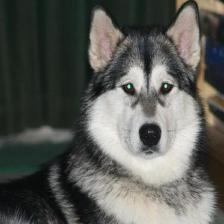
\includegraphics[width=2.8cm]{../dataset/test/n02110063-malamute/n02110063_11838.jpg}\hfill 
    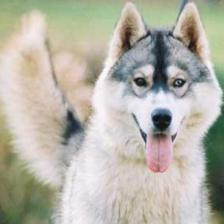
\includegraphics[width=2.8cm]{../dataset/test/n02109961-Eskimo_dog/n02109961_623.jpg}\hfill 
    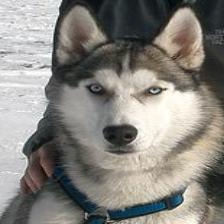
\includegraphics[width=2.8cm]{../dataset/test/n02110185-Siberian_husky/n02110185_7564.jpg} 
    \caption{De gauche à droite, un Malmute, un Eskimo et un Husky}
    \label{1}
\end{figure} 

\subsection{Travaux antérieurs}
L'article \textit{Using Convolutional Neural Networks to Classify Dog Breeds}
~\cite{fcdh_FinalReport} est un incontournable. Concrètement, les auteurs
proposent  deux architectures différentes capables de différencier les petites
variations entre les races. Le premier modèle est basé sur l'architecture de 
LeNet, dont chaque couche de convolution est un filtre avec 2 paramètres : le 
nombre de pixels qu’elles prennent en entrée et le nombre de canaux en sortie.
Le second modèle reprend l'architecture de GoogLeNet, dont chaque couche de
convolution est une combinaison de filtres eux-mêmes composés de réseaux de
neurones.

Un autre papier intéressant est \textit{Dog Breed Identification}. 
~\cite{output} Il y est présenté un projet ayant pour but de prédire les races
des chiens à partir d’images. Ce projet utilise des techniques d’apprentissage
automatique et de vision par ordinateur. Un réseau de neurones convolutionnel
permet, dans un premier temps, d’identifier les points clés des visages des 
chiens. Ensuite, des descripteurs SIFT (\textit{Scale-Invariant Feature
Transform}) et des histogrammes de couleur utilisent ces points clés pour
extraire des \textit{features}. Enfin, un classificateur de type machine à
vecteur de support (SVM) prédit la race du chien avec une précision de 52\%. Il
est à noter que dans 90\% des cas, la race du chien à trouver est présente dans
les 10 prédictions les plus probables depuis 133 races au total dans la base de 
données. Ces performances sont supérieures à ce que peuvent faire la plupart
des humains.

Dans ce travail, nous nous inspirons d'un modèle proposé par le premier article.
En effet, la simplicité d’architecture et leurs performances sont totalement
adaptées aux contraintes que nous rencontrons. Nous allons ajouter un algorithme
qui applique une étiquette sur l'image.

\section{Approche théorique}
% Un résumé de l'approche théorique formant la base du sujet du projet.

\subsection{GoogLeNet}
Le modèle GoogLeNet créé par Google possède le mot LeNet dans son nom, car il
rend hommage à son prédécesseur LeNet qui est un des premiers modèles de
convolution à apporter de réelles prédictions de contenu d’images. Avant le
développement de GoogLeNet,  beaucoup d’autres modèles de convolution ont vu le
jour comme AlexNet, mais le modèle de Google reste celui qui a le pourcentage
d’erreur le plus bas et qui est donc le plus performant tel que présenté
sur la figure \ref{2} ~\cite{tsang_2018}.

\begin{figure}[htbp]
    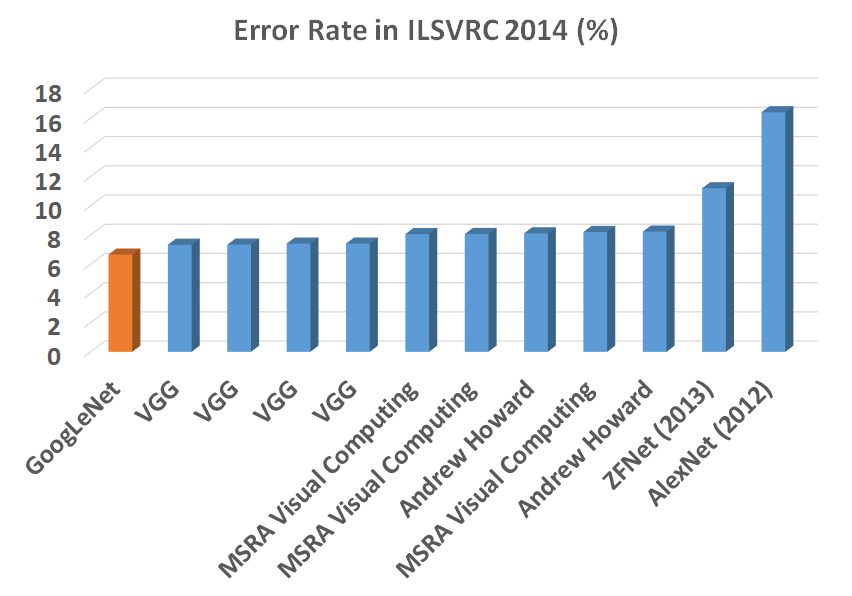
\includegraphics[width=8.4cm]{./figures/Figure1.png} 
    \caption{Les modèles participants à l'ILSVRC 2014}
    \label{2} 
\end{figure} 

L'architecture de ce réseau GoogleNet est très différente des précédents réseaux
existants. Il contient des convolutions $1\times 1$ au milieu du réseau et le
regroupement moyen global est utilisé à la fin du réseau au lieu d’utiliser des
couches entièrement connectées. Ces deux techniques sont extraites d’un autre
article intitulé \textit{Network In Network}. ~\cite{lin2013network} Une autre
technique, appelée module de création, consiste à avoir différentes tailles ou
types de convolutions pour la même entrée. Ensuite, on empile toutes les 
sorties. Nous verrons plus en détail chacune de ces techniques.

\subsection{Convolution $1\times 1$}
Dans GoogLeNet, la convolution $1\times 1$ est utilisée comme module de
réduction de dimension pour réduire le calcul. En réduisant le goulot
d'étranglement du calcul, la profondeur et la largeur peuvent être augmentées.
Prenons un exemple simple pour illustrer cela. Supposons que nous devons
effectuer une convolution $5\times 5$ sans utiliser la convolution $1\times 1$
tel qu'illustré à la figure \ref{3} ~\cite{tsang_2018}.

\begin{figure}[htbp]
    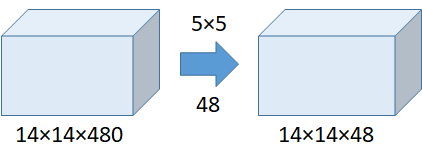
\includegraphics[width=8.4cm]{./figures/Figure2.png} 
    \caption{Convolution de 112,9 millions opérations}
    \label{3} 
\end{figure} 

Voyons maintenant le nombre d’opérations effectuées si l’on ajoute une
convolution $1\times 1$ comme sur la figure \ref{4} ~\cite{tsang_2018}.

\begin{figure}[htbp]
    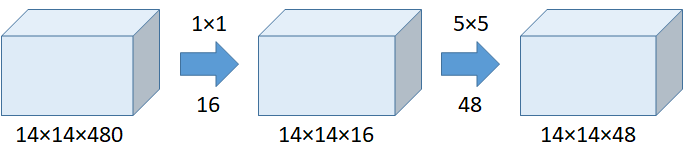
\includegraphics[width=8.4cm]{./figures/Figure3.png} 
    \caption{Convolution de 5,3 millions opérations}
    \label{4} 
\end{figure} 

Les deux sous-modèles de convolution ci-dessus donnent le même résultat et sont
donc équivalents. Cependant, lorsqu’on utilise la convolution $1\times 1$ en
plus on effectue beaucoup moins d’opérations ce qui est moins couteux. Ainsi,
la convolution $1\times 1$ aide à réduire la taille du modèle, ce qui peut
également aider à réduire les problèmes de généralisation.

\subsection{Inception}
Auparavant, comme avec AlexNet et VGGNet, la taille du filtre de convolution
était fixée pour chaque couche. Mais avec le module Inception, les filtres de
convolution $1\times 1$,  $3\times 3$ et  $5\times 5$ ainsi que la couche
\textit{maxpooling} sont toutes appliquées à la sortie de la couche de neurones
précédente et chaque résultat de chacune de ces couches est envoyé vers une
couche de concaténation qui regroupe toutes ces sorties en un seul résultat.
L’architecture de ce module est de la forme représentée à la figure \ref{5}.
 ~\cite{43022}

\begin{figure}[htbp]
    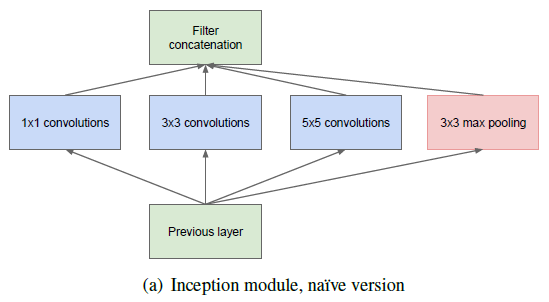
\includegraphics[width=8.4cm]{./figures/Figure5.png} 
    \caption{Inception Naïf}
    \label{5} 
\end{figure} 

Finalement, si on décide de regrouper et d’utiliser la convolution $1\times 1$
dans notre module Inception, on réduit la dimension des couches $3\times 3$
et $5\times 5$ pour qu’elles soient moins couteuses. On garde donc la variété
de résultats qu’offre l’assemblage de couches de convolution de différentes
tailles tout en prenant soin de réduire les dimensions pour éviter une surcharge
des opérations et, par la même occasion, les problèmes de généralisation comme
dans la figure \ref{6}. ~\cite{43022}

\begin{figure}[htbp]
    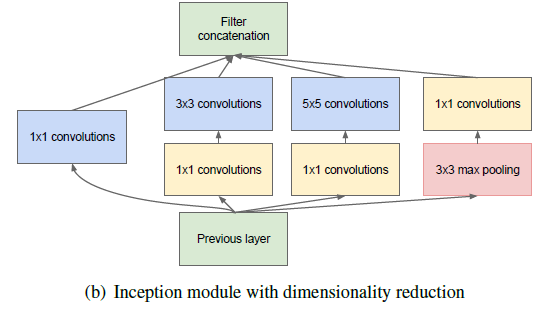
\includegraphics[width=8.4cm]{./figures/Figure6.png} 
    \caption{Inception réduit}
    \label{6} 
\end{figure} 

\subsection{Regroupement moyen global}
Dans la plupart des CNN classiques et déjà réalisées, on utilise une couche
pleinement connectée (FC) à la fin du réseau à la sortie de la dernière couche
de convolution ou de \textit{pooling} en reliant toutes les entrées à toutes les
sorties qui sont égales au nombre de classes que l’on veut classifier à l’aide
notre modèle. Dans notre cas, nous avons 120 classes qui représentent les 120
races de chiens différentes. Néanmoins, GoogLeNet n’utilise pas de couche FC à
la fin pour la classification, mais bien une couche de regroupement moyen global
(GAP) qui consiste à calculer, pour chaque entrée, une moyenne de probabilité
qu’il va envoyer directement à la sortie. Il n’y aura donc aucune matrice de
poids à apprendre comme pour un réseau FC. Le concept du GAP est représenté à la
figure \ref{7}. ~\cite{tsang_2018}

\begin{figure}[htbp]
    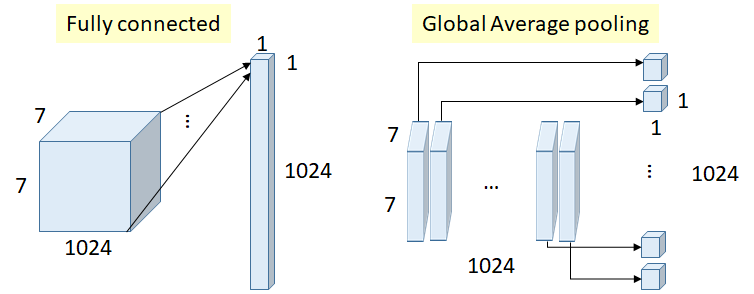
\includegraphics[width=8.4cm]{./figures/Figure4.png} 
    \caption{Comparaison de FC et GAP}
    \label{7} 
\end{figure} 

On voit donc que le réseau FC utilise toutes les entrées pour déterminer une
sortie alors que le GPA utilise une entrée par sortie par rapport à un calcul 
des entrées moyennes. Le réseau GPA est donc moins couteux. De plus, une étude
des auteurs a confirmé qu'un passage de la couche FC à la couche GPA améliore la
précision du GoogLeNet de 0,6\% ce qui est remarquable. ~\cite{tsang_2018}

\subsection{Méthodologie}
Dans le contexte de la pandémie, nous devons limiter le projet à quelque chose 
de simple, qui permet toutefois de comprendre le fonctionnement d'un CNN 
moderne en profondeur. Ainsi, nous allons nous limiter à une seule architecture.

Premièrement, nous avons évalué s'il était possible d'ajouter des étiquettes à une
image dans ses métadonnées à l'aide du langage Python. Nous avons trouvé la
librairie IPTCInfo qui permet de faire cette tâche aisément.

Ensuite, nous avons cherché un jeu de données pour entrainer notre modèle. Les
images retenues proviennent du \textit{Stanford Dogs Dataset}. 
~\cite{KhoslaYaoJayadevaprakashFeiFei_FGVC2011} Le fait que les clichés soient
présents dans des répertoires nommés par la race permet facilement de retrouver
l'étiquette pour faire l'entrainement supervisé. Aussi, le fait que le jeu de
données soit différent de l'article permet d'explorer davantage les impacts du
jeu de données  par rapport au modèle.

Pour concevoir le modèle, nous utilisons un GoogLeNet comme dans l'article 
\textit{Using Convolutional Neural Networks to Classify Dog Breeds} 
~\cite{output}. Ainsi, il nous a été utile de consulter l'article de Google,
\textit{Going deeper with convolutions} ~\cite{43022}, afin de bien comprendre
le fonctionnement du réseau.

Le modèle que nous avons implémenté en python à l’aide de couches de Pytorch
est fortement inspiré du modèle GoogLeNet auquel nous avons décidé d’ajouter des
couches de normalisation par sous-ensemble afin d’améliorer l’entrainement. En
effet, nous avons implémenté une classe Inception composée de quatre branches de
séparation du transformer, qui ont leur sortie regroupée à la fin de la classe.
De plus, nous avons aussi une classe GoogLeNet composée de trois couches de
convolution suivies chacune d'une couche de normalisation par sous-ensemble puis
d’une couche ReLU et enfin d’une couche de \textit{pooling}. L'architecture
implémentée est représentée par la figure \ref{8}. L'architecture est disponible
dans le fichier googlenet.py sur le dépôt GitHub disponible à cette adresse :
\url{https://github.com/Anteige/INF8225}

\begin{figure}[htbp]
    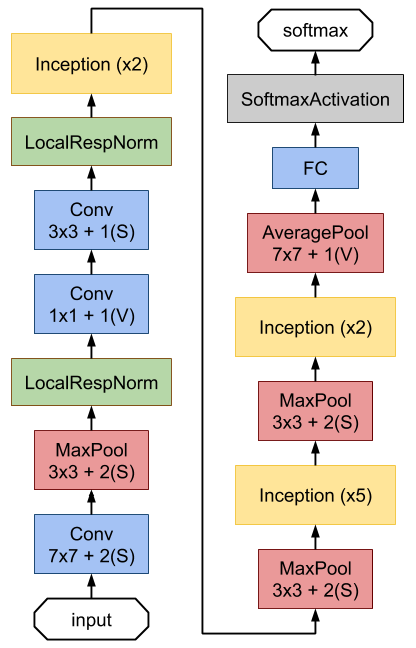
\includegraphics[width=8.4cm]{./figures/Figure7bis.png} 
    \caption{Architecture implémentée}
    \label{8} 
\end{figure} 

\section{Discussion}
% Discussion de nos expériences. Incluant des figures, des tableaux de nos résultats.

\subsection{Entraînement}
Afin de réaliser l’entrainement sur notre implémentation de GoogLeNet, nous
avons choisi comme input 12000 images d’entrainement, soit 1000 images par race
de chien, de taille $3\times 244 \times 244$. Chaque dimension représente
respectivement, la couleur RBG, la longueur et la largeur. Ce jeu de données est
importé de Kaggle. Nous l’avons choisi, car il est plutôt récent et les
résultats des entrainements sur ce jeu de données à ce jour sont loin d’être
performants. Pour ce qui est du modèle, nous avons choisi, à l’aide d’un
ensemble de validation, des taux d’apprentissages égaux à 0,07 et 0,0005 ainsi
qu'un momentum de 0,0005. L’algorithme d’optimisation employé est ADAM et la
fonction de perte utilisée pour mesurer l’erreur après chaque mise à jour du
modèle est l'entropie croisée.

Nous avons effectué plusieurs essais en variant le taux d'apprentissage, le
nombre d'itérations et l'utilisation, ou non, d'une optimisation ADAM. Pour
chaque essai, nous avons noté le score en top1 et en top10. Pour des fins de
comparaisons, seule la moyenne a été retenue.

\subsection{Résultats}
\begin{table}[htbp]
\centering
\begin{tabular}{lrr}  
\toprule
Nombre d'itérations & top1 (\%) & top10 (\%) \\
\midrule
1000 & 0.89 & 2.60 \\
         & 0.87 & 2.66 \\
         & 0.72 & 2.45 \\
         & 0.84 & 2.67 \\
         & 0.82 & 2.53 \\
         & $\mu = 0.83$ &  $\mu = 2.58$ \\
300   & 0.65 & 2.38 \\
         & 0.73 & 2.44 \\
         & 0.75 & 2.42 \\
         & 0.80 & 2.37 \\
         & 0.59 & 2.30 \\
         & $\mu = 0.71$ &  $\mu = 2.38$ \\
200   & 0.78 & 2.24 \\
         & 0.84 & 2.38 \\
         & 0.84 & 2.47 \\
         & 0.71 & 2.40 \\
         & 0.80 & 2.59 \\
         & $\mu = 0.79$ &  $\mu = 2.41$ \\
100   & 0.77 & 8.11 \\
         & 0.73 & 8.25 \\
         & 0.63 & 8.23 \\
         & 0.78 & 8.37 \\
         & 0.80 & 8.59 \\
         & $\mu = 0.74$ &  $\mu = 8.31$ \\
\bottomrule
\end{tabular}
\caption{Performances avec un taux d'apprentissage de 0,0005}
\label{tab:1}
\end{table}

\begin{table}[htbp]
\centering
\begin{tabular}{lrr}  
\toprule
Nombre d'itérations & top1 (\%) & top10 (\%) \\
\midrule
1000 & 0.89 & 2.60 \\
         & 0.87 & 2.66 \\
         & 0.72 & 2.45 \\
         & 0.84 & 2.67 \\
         & 0.82 & 2.53 \\
         & $\mu = 0.83$ &  $\mu = 2.58$ \\
\bottomrule
\end{tabular}
\caption{Performances avec un taux d'apprentissage et un L2 de 0,0005}
\label{tab:2}
\end{table}

\begin{table}[htbp]
\centering
\begin{tabular}{lrr}  
\toprule
Nombre d'itérations & top1 (\%) & top10 (\%) \\
\midrule
50 & 0.96 & 8.86 \\
     & 0.73 & 8.68 \\
     & 0.70 & 8.40 \\
     & 0.63 & 8.54 \\
     & 0.84 & 8.96 \\
     & $\mu = 0.77$ &  $\mu = 8.69$ \\
\bottomrule
\end{tabular}
\caption{Performances avec un taux d'apprentissage de 0,07}
\label{tab:3}
\end{table}

\subsection{Interprétation des résultats}
Dans le tableau \ref{tab:1}, on voit que les résultats de l’entrainement avec
beaucoup d’itérations sont moins bons à partir de 100 itérations. En effet, on
constate que même si l’erreur de la fonction de cout continue à diminuer après
100 itérations et qu’elle devient acceptable à partir de 500 itérations, les
résultats ne vont pas dans ce sens, ce qui nous laisse penser que le modèle
passe en surapprentissage au bout de 100 itérations d’entrainement.

Dans le tableau \ref{tab:2}, on constate que l'application d'un L2 ...

Dans le tableau \ref{tab:3}, ... TODO

\subsection{Observations}
Nous avons remarqué que la perte de la fonction de cout diminue très lentement
lors de la phase d’entrainement. En effet, le modèle classique GoogLeNet réalisé
par Google s’est entrainé sur une multitude d’objets et d'êtres vivants
différents. Il a donc pu apprendre chaque \textit{freatures} différente selon
chaque entrée. Dans notre cas, nous avons décidé de ne pas utiliser la version
préimplémentée du modèle de Google, en l'important depuis la libraire Pytroch,
mais de la réimplémenté nous même et surtout de le refaire son entrainement à
partir de zéro. Notre modèle doit donc apprendre à reconnaitre différentes races
de chiens uniquement.

Or, même si les chiens que nous lui avons donnés en entrée sont de races
différentes, ils ont quand même énormément de similitudes, comme un museau, de
longues oreilles, une posture à quatre pattes, etc. Le modèle de convolution
extrait donc souvent des caractéristiques similaires à chaque fois même si les
chiens sont de race différente ce qui fait toute la complexité et la difficulté
de notre apprentissage c’est pourquoi nous avons décidé d’ajouter la dimension
de couleur RBG dans nos images d’entrée, car nous nous sommes dit que
l’apprentissage des couleurs pourrait aider à reconnaitre différentes races de
chiens qui sont souvent de couleurs différentes. C’est d’ailleurs pour cela que
l’article que nous avons étudié pour faire ce projet a obtenu en résultat une
précision de 10\% sur la reconnaissance de race de chiens en utilisant le modèle
de Google avec un jeu de données certes différent qui est ImageNet. Il nous a
donc semblé intéressant de tester notre propre implémentation du modèle de
Google sur ce jeu de données afin de voir s'il arrive à obtenir de bons résultats
en entrainant notre modèle uniquement sur des chiens.

Pour pallier le fait que la perte diminue très lentement, nous avons décidé de
laisser le modèle s’entrainer pendant un nombre d’itérations d’entrainement de
plus en plus grand. Nous sommes allés jusqu’à tester plus de 1000 itérations, ce
qui a pris 18 heures environ.

\section{Analyse}
% Une analyze critique de l'approche que vous avez utilisée pour apprendre le sujet que vous avez sélectionné.
Nous avons donc une meilleure précision que l’article que nous avons étudié,
en utilisant le même modèle GoogleNet avec 3 couches d'Inception. Cela est dû,
selon nous, à l’ajout de couches de normalisation par sous-ensemble ainsi qu’à
l’entrainement exclusif sur des chiens, mais aussi grâce à notre jeu de données.
La précision est néanmoins loin d’être bonne et utilisable comme nous le
souhaitions. En effet, le but de notre projet était de modifier les mots-clés de
chaque image selon la prédiction de notre modèle. Même si nous sommes arrivés à
une perte sur une erreur d’entrainement suffisamment petite, le modèle a encore
du mal à généraliser sur l’ensemble de tests à cause des similitudes qui
existent entre les races de chiens. Dans l'article que nous avons décidé
d'implémenté, on trouves des résultats de modèles GoogleNet composée de 3, 4, 6
et 7 couches inceptions respectivements. L'implémentation que nous avons décidé
d'implémenter est le googleNet à 3 couches inceptions. Par rapport à cela nous
pouvons affirmer que notre modèle GoogleNet donne des résultats
significativement meilleurs que l'article. Cependant, cette performance est
insuffisante pour une classification proche de l'être humain.

Pour en revenir à l’analyse de nos tableaux, on voit que les résultats de
l’entrainement avec beaucoup d’itérations sont moins bons à partir de 100
itérations. En effet, on constate que même si l’erreur de la fonction de cout
continue à diminuer après 100 itérations et qu’elle devient acceptable à partir
de 500 itérations, les résultats ne vont pas dans ce sens, ce qui nous laisse
penser que le modèle passe en surapprentissage au bout de 100 itérations
d’entrainement. 

Afin de mieux comprendre ce phénomène, posons-nous la question suivante :
qu’est-ce que le modèle veut apprendre ? Et bien notre modèle est principalement
basé sur des convolutions, il cherche donc à apprendre des filtres de
convolution afin de reconnaitre les caractéristiques d’une image afin de pouvoir
la classifier selon ces caractéristiques. De plus, à l’aide des couches de
pooling, il cherche à réduire l’information inutile qui n’est pas en rapport
avec les caractéristiques qu’il souhaite apprendre. Or, sachant que les chiens
ont tous des caractéristiques similaires, notre modèle va apprendre ces
caractéristiques minimisées, par les couches de pooling, et ne saura donc plus
les utiliser pour classifier les races de chiens. En somme, augmenter le nombre
d’itérations de l’apprentissage ne nous aidera pas à mieux apprendre ces
caractéristiques, qui diffèrent selon chaque race de chien, mais bien au
contraire, notre GoogLeNet va vite tomber dans le surapprentissage, car il va
apprendre sans cesse des caractéristiques qui ne lui apporteront pas
suffisamment de détails pour classifier les races de chiens de notre jeu de
données. 

En conclusion de cette analyse, nous pensons qu’il serait justifiable de réduire
au minimum les tailles des filtres de convolution avec les couches de pooling
car ceux-ci font perdre de l’information précieuse. Le problème avec cette
méthode est que l’information à traiter sera en conséquence plus grande et nous
aurons besoin d’un réseau beaucoup plus profond que ceux utilisables à notre
niveau d’un point de vue matériel et temporel. Un jeu de données plus grand
pourrait également aider dans ce sens pour un apprentissage de détail plus
profond et pour un risque de surapprentissage plus faible.

%% The file named.bst is a bibliography style file for BibTeX 0.99c
\bibliographystyle{named}
\bibliography{rapport}

\end{document}

